\chapter{RADICI DI UN EQUAZIONE}
\section{Esercizio 5}

\textit{\textbf{Descrizione:} Scrivere function Matlab distinte che implementino efficientemente i seguenti metodi per la ricerca degli zeri di una funzione:
\begin{itemize}
\item metodo di bisezione 
\item metodo di Newton
\item metodo delle secanti 
\item metodo delle corde
\end{itemize}
Detta $x_{i}$ l'approssimazione al passo i-esimo, utilizzando come criterio di arresto $\left | \Delta x_{i} \right |\leq tol \cdot (1 + \left | x_{i} \right |)$ essendo $tol$ una opportuna tolleranza specificata in ingresso.}\newpage
\emph{Soluzione: }\\~\\
\textbf{il metodo di bisezione:}
\\~\\
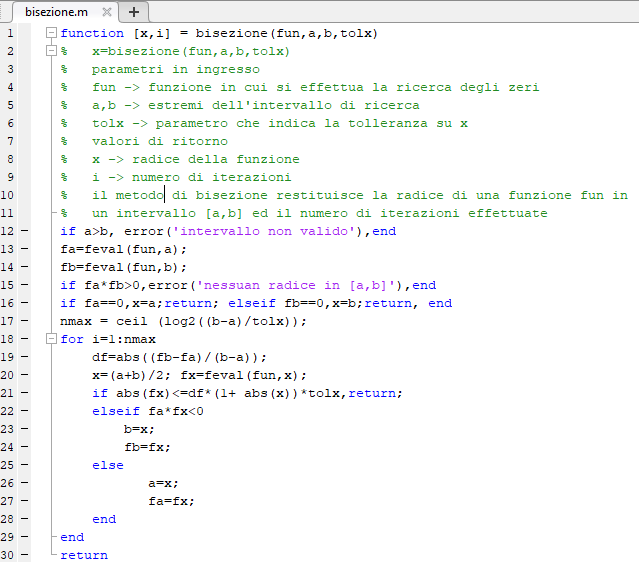
\includegraphics[width=1.3\linewidth]{img/bisezione} \newpage
\textbf{il metodo di Newton:}
\\~\\
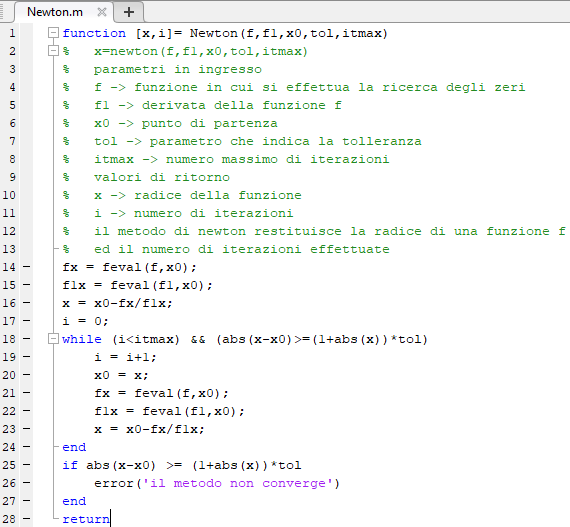
\includegraphics[width=1.3\linewidth]{img/newton}\newpage
\textbf{il metodo delle secanti:}
\\~\\
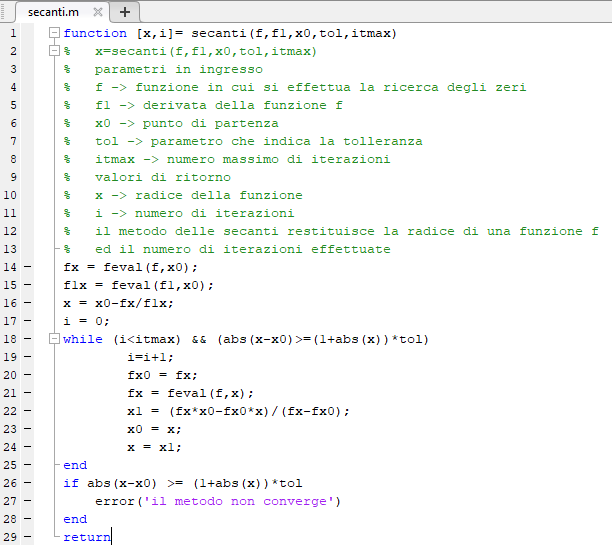
\includegraphics[width=1.3\linewidth]{img/secanti}\newpage
\textbf{il metodo delle corde:}
\\~\\
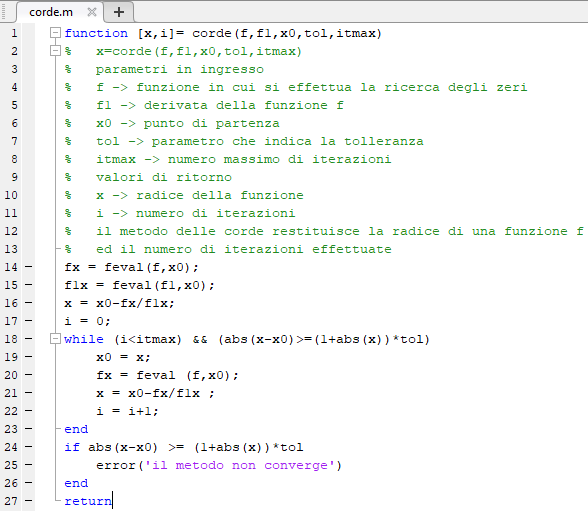
\includegraphics[width=1.3\linewidth]{img/corde}\newpage